\section{Funktionenfolgen und deren Konvergenz}
\subsection{Funktionenfolgen und deren Konvergenz}
Ist $ \Omega \subset \R  $ nichtleer und für jedes $ n \in \N  $ eine Funktion $ f_n : \Omega \to \R  $ definiert, so nennen wir $ (f_n) $ eine Funktionenfolge

\begin{subexample}
	Sei für $ n \in \N \quad f_n : \Omega \to \R , x \mapsto x^n $. z.B.
	\begin{enumerate}[label=\arabic*.]
		\item $ f_1: \Omega \to \R , x \mapsto x $ 
		\item $ f_2: \Omega \to \R , x \to x^2 $
		\item usw.
	\end{enumerate}
\end{subexample}

\begin{subdefinition}[Punktweise Konvergenz]
	Sei $ \Omega \subset \R  $ nichtleer und $ f, f_1, f_2, \dotsc: \Omega \to \R  $.\\
	Wir sagen $ (f_n) $ \textbf{konvergiert punktweise gegen} $ f $, falls $ \forall x \in R $ die Folge $ (f_n(x)) $ gegen $ f(x) $ konvergiert.\\
	Gibt es ein $ f:\Omega\to \R  $, so dass $ (f_n) $ punktweise gegen $ f $ konvergiert, so nennen wir $ (f_n) $ \textbf{punktweise konvergent}.\\
	Wir nennen dann $ f $ \textbf{Grenzfunktion} von $ (f_n) $.\\
	Das bedeutet:
	\[
		\forall x \in \Omega: \forall \varepsilon > 0 : \exists N \in \N : \forall n \geq N: |f_n(x) - f(x) | < \varepsilon 
	\]
\end{subdefinition}

\begin{subexample}
	Sei $ \Omega = [0, 1] $. Wir betrachten $ f_n: \Omega \to \R  $ mit $ f_n(x) = x^n, x \in [0, 1] $.\\
	Ist $ x \in [0, 1) $, so $ \lim_{n \to \infty} f_n(x) = 0 $. Hingegen $ \lim_{n \to \infty} f_n(x) = 1 $ für $ x = 1 $.
	Also konvergiert $ (f_n) $ punktweise gegen
	\[
		f: \Omega \to \R \text{ mit } f(x) \coloneqq \begin{cases}
			0 & \text{für } 0\leq x<1\\
			1 & \text{für } x = 1
		\end{cases}
	\]
\end{subexample}
\begin{figure}[!ht]
	\centering
	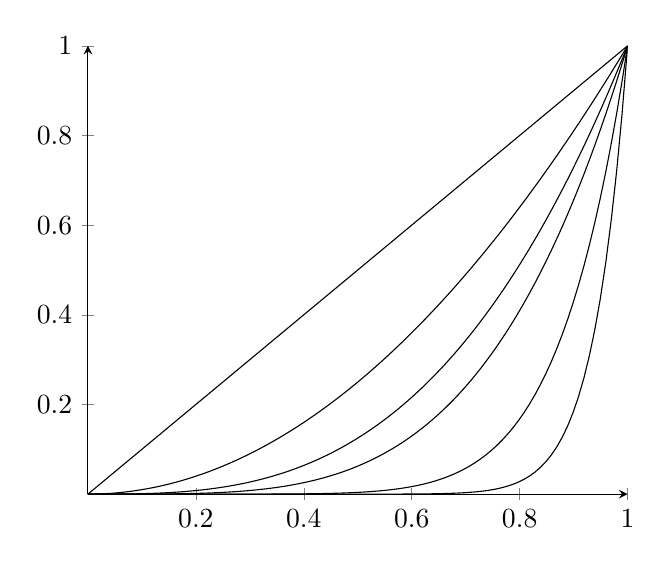
\begin{tikzpicture}
		\begin{axis}[
			xmin= 0, xmax= 1,
			ymin= 0, ymax = 1,
			axis lines = middle,
		]
			\addplot[domain=0:1, samples=100]{x};
			\addplot[domain=0:1, samples=100]{x^2};
			\addplot[domain=0:1, samples=100]{x^3};
			\addplot[domain=0:1, samples=100]{x^4};
			\addplot[domain=0:1, samples=100]{x^8};
			\addplot[domain=0:1, samples=100]{x^16};
		\end{axis}
	\end{tikzpicture}
	\begin{tikzpicture}
		\begin{axis}[
			xmin= 0, xmax= 1,
			ymin= 0, ymax = 1,
			axis lines = middle,
		]
			\addplot[domain=0:1, samples=100, color = blue]{0};
			\addplot[color = blue, mark = *, only marks] coordinates{(1,1)};
			\draw[dotted, color = blue] (axis cs:1,0) --(axis cs:1,1);
		\end{axis}
	\end{tikzpicture}
	\caption{Definition 8.1.2}
	\label{Definition8.1.2}
\end{figure}

\begin{subdefinition}
	Sei $ \Omega \subset \R  $ nichtleer und $ f, f_1, f_2, \dotsc : \Omega \to \R  $.
	Wir sagen $ (f_n) $ {\color{yellow} konvergiert gleichmäßig gegen} f, falls für jedes $ \varepsilon > 0 $ ein $ N \in \N  $ existiert, sodass $ |f(x) - f_n(x)| < \varepsilon  $ f.a. $ x \in \Omega $ und alle $ n \geq N $ gilt.\\
	Das bedeutet:
	\[
		\forall \varepsilon > 0: \exists N \in \N \forall n \geq N : \forall x \in \Omega: |f_n(x) - f(x)| < \varepsilon .
	\]
\end{subdefinition}

\begin{sublemma}
	Sei $ \Omega \subset \R  $ nichtleer und $ f, f_1, f_2, \dotsc : \Omega \to \R  $ so, dass $ (f_n) $ gleichmäßig gegen $ f $ konvergiert.
	Dann konvergiert $ (f_n) $ auch punktweise gegen $ f $.
\end{sublemma}

\begin{subexample}
	Die Folge aus Beispiel \ref{8.1.3} konvergiert nicht gleichmäßig.\\
	Sei $ 1 > \varepsilon > 0, N \in \N  $ beliebig. Setzte $ x \coloneqq \sqrt[n]{\varepsilon }   $. Dann ist $ x_0 \in (0, 1) $ und $ f_n(x_0) = \varepsilon  $, d.h. $ |f_n(x_0) - f(x_0)| = |f_n(x_0)| = \varepsilon \geq \varepsilon  $
\end{subexample}

\begin{subtheorem}
	Sei $ \Omega \subset \R  $ nichtleer und $ f_1, f_2, \dotsc : \Omega \to \R  $ stetige Funktionen.
	Konvergiert $ (f_n) $ gleichmäßig gegen $ f: \Omega \to \R  $, so ist $ f $ stetig.
\end{subtheorem}

\begin{subproof*}[Theorem \ref{8.1.7}]
	Sei $ x_0 \in \Omega $ und $ \varepsilon > 0 $ beliebeig. Dann finden wir wegen glm. Konv. ein $ N \in \N $
	mit $ |f_n(x) - f(x)| < \frac{ \varepsilon  }{ 2 }  $ ...
\end{subproof*}

